\section{Konseptet}\label{sec:konsept}

\subsection{Introduksjon: Garbage Alert}

			\begin{figure} [here]
				\begin{center}
					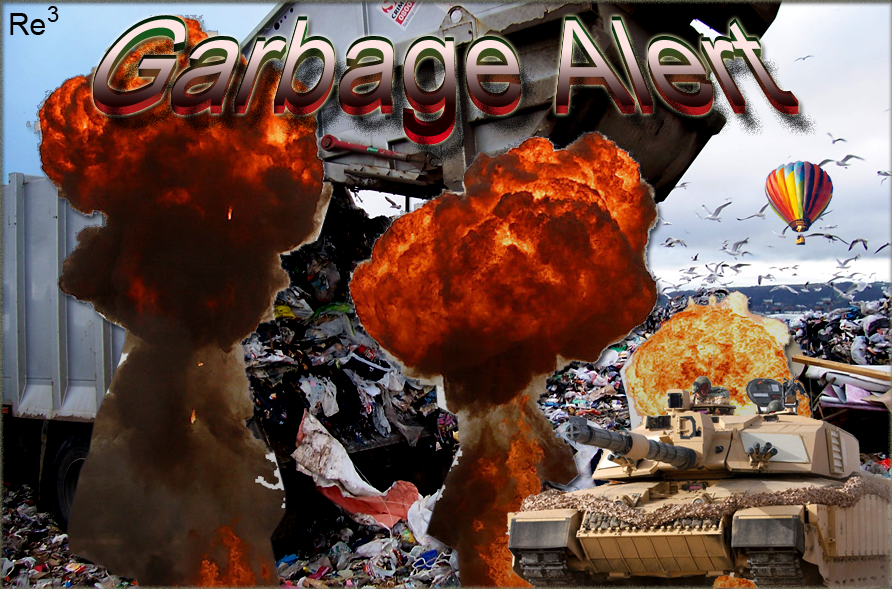
\includegraphics[scale=0.5]{images/splashscreen}
				\end{center}
			\caption{Garbage Alert splash screen}
		\end{figure}

Garbage Alert er strategispillet der du bestemmer verdens skjebne ved å gjenvinne og krige med søppel. Spillet har resirkulering i sentrum samtidige som det skal være et underholdende strategispill for deg mellom 9 og 99 år. 

Man starter på en øy overfyllt med søppel. Målet med spillet er å bli kvitt søppelet. Ved å gjenvinne avfallet får man ulike muligheter til å bombandere de andre spillerne, forsvare sin egen øy, for så å stå igjen som vinneren på en øy uten søppel, eller som eneste spiller i live.

Spillet er utviklet av en gruppe studenter på NTNU i faget Eksperter i Team. Spilldesignerne går under navnet Re3. Re3 består av Andreas Røysland Aarnes, Trond Kjetil Bremnes, Christian Aleksander Lysne, Kjetil Mehl og Ina Sander Pedersen.

Målet med dette avsnittet er å gi deg et innblikk i det utviklede spillkonseptet,
hvilke spillaspekter som er tatt med og spilldynamikken.

%Garbage Alert er et sanntids strategispill for mobile enheter. Hver
%spiller blir tildelt en øy dekket med søppel. En øy består av en
%gjenvinningsstasjon, en våpenstasjon og en forsvarssone.
%Gjenvinningsstasjonen har som oppgave å transformere øyas søppel om til
%ressurser. Disse ressuresene kan brukes til å kjøpe våpen,
%forsvarsmurer, utvinne nye ressurser og oppgradere
%gjennvinningsstasjonen. Mulige oppgraderinger for gjenvinningsstasjonen
%er raskere gjennvinning og større kapasitet for inntak av søppel. Våpen
%brukes til å skyte søppel på motstandernes øyer, og forsvarsmuren har
%som oppgave å blokkere slike angrep. 

%vinnsenarioet er å bli den første til å kvitte seg med alt søppelet på
%øyen sin. Den andre måten å vinne på er å skyte i stykker motstandernes
%gjenvinningsstasjon. Hvis en øy mister gjenvinningsstasjonen sin, vil
%den bli oversvømt med søppel og synke ned i havet. Dermed kan spilleren
%velge om han/hun vil fokusere på å forbedre sin egen øy eller ødelegge
%for andre. 

\subsection{Spillanalyse}

Garbage Alert er et flerspiller sanntidsstrategispill, men muligheten for å spille alene mot pc-en finnes også. 

Når man starter spillet har man følgende elementer:

\begin{itemize}
	\item et resirkuleringssenter
	\item en våpenstasjon
	\item en forsvarssone
	\item 10 enheter med papp i inventaret
	\item 1000 enheter med søppel
	\item muligheten til å gjenvinne papp fra søppelet. Gjenvinningsgraden er 10\%
	\item muligheten til å bruke papp til å bygge våpen (papirfly) og forsvar (pappmur)
	\item muligheten til å oppgradere gjenvinningsgraden til 20\%
	\item muligheter for oppgraderinger av gjenvinningsstasjon slik at man også får gjenvinnet plast eller tre.
\end{itemize}

Jo flere typer ressurser man får gjenvinnet fra søppelet, jo flere muligheter har man får mer avanserte våpen, forsvar og oppgraderinger. Man starter med å kun gjenvinne papp. Figur xx viser mulighetene man har for å oppgradere resirkuleringssenteret slik at man får muligheten til å gjenvinne andre ressurser. For eksempel hvis man skal oppgradere til stål, må man først oppgradere til plast. For å oppgradere til titan kreves det at alle andre oppgraderinger allerede er utført.

			\begin{figure} [here]
				\begin{center}
					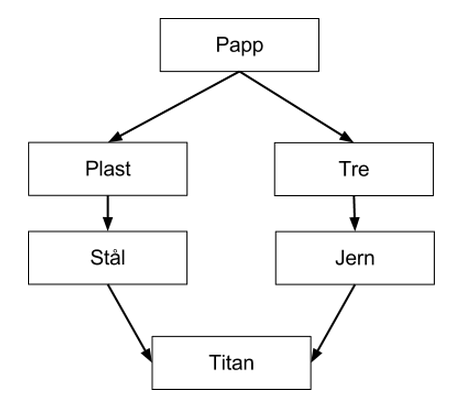
\includegraphics[scale=0.5]{images/oppgraderingstre}
				\end{center}
			\caption{Ressursoppgraderinger}
		\end{figure}
		
		
De sentrale spillelementene består av å samle inn søppel til resikulerings vil være samling, ressursforvaltning, valg av våpen og forsvar, samt timing av våpenbruk. Spillinnholdet vil hovedsaklig være Pure Play (Usikker på dette innebærer det jeg tror), der målet er å få spilleren til å ha det gøy, men det vil også være elementer av realisme da det spilleren foretar seg vil virke inn på både lokalt og globalt miljø. Det vil være en lineær spillsekvens (Er usikker på denne fordi jeg ikke finner noen  spillsekvenstype som passer??) der spilleren får tilgang til nye våpentyper og forsvarsmuligheter etterhvert som krav for hver enkelt oppgradering er nådd. For at spillet skal få et lekent og fristende utseende har vi valgt en type tegneseriestil som vil gjøre nettopp dette. (Husker ikke om vi har vi diskutert dette, og hva vi kom fram til?)
\\
Game Reference / Spillreferanse: Sjønner ikke helt hva som skal være med her, spillstrategi, spillinnlevelse, referanser
\\
Spillteknisk: Den tekniske formen (technical form) på spillet er flat 2D grafikk (Eller er jeg helt på bærtur??) der visningen for spilleren vil være i et ovenfra-ned perspektiv (top-down perspective). Programvareplattform er Java (Eller ikke?) og spillet er hovedsaklig tenkt for mobilenheter.

Spillbeskrivelse: Spillets sjanger er valgt til flerspiller sanntidsstrategi, men det vil også være mulighet for å spille alene mot computer. (Usikker på om vi ble enig om at dette skulle være mulig?) Viktige spillelementer vil være samling, ressursforvaltning, valg av våpen og forsvar, samt timing av våpenbruk. Spillinnholdet vil hovedsaklig være Pure Play (Usikker på dette innebærer det jeg tror), der målet er å få spilleren til å ha det gøy, men det vil også være elementer av realisme da det spilleren foretar seg vil virke inn på både lokalt og globalt miljø. Det vil være en lineær spillsekvens (Er usikker på denne fordi jeg ikke finner noen  spillsekvenstype som passer??) der spilleren får tilgang til nye våpentyper og forsvarsmuligheter etterhvert som krav for hver enkelt oppgradering er nådd. For at spillet skal få et lekent og fristende utseende har vi valgt en type tegneseriestil som vil gjøre nettopp dette. (Husker ikke om vi har vi diskutert dette, og hva vi kom fram til?)\\ 


\subsection{Spillatmosfære}

This is where it is best to have a mood board or a clear description of the game’s style. 

This is a good place to start interacting with a graphic designer.\\

Atmosphere Mood Board\\
Character  Units Sketch and Description\\
A Level(Locations) Sketch and Description\\
Audio Description

\subsection{Game Play}

Using this outline to create a descriptive paragraph about how the game is played. 

The idea is that you want the person imagine they are actually playing the game.

Do not use Generic names when writing about the game play. 

Example: No one wants to here that enemy 1 will have more hit points than enemy 2. Instead we should talk about how the Lazarus Fighter has more armour than Apollo Fighter.

This outline will vary according to the type of game. \\
Opening the game application\\
Game Options \\
Story Synopsis\\
Modes\\
Game Elements\\
Game Levels\\
Player’s Controls\\
Winning\\
Losing\\
End\\
Why is all this fun?\\
\\

\subsection{Nøkkelfunksjoner}

Key features are a list of game elements that are attractive to the player.

It is a good idea to talk about the key features with someone from marketing.\\
Number of Levels\\
Number of Enemies or Characters (Example: 12 characters or amount of enemies, end bosses)\\
Time of Game Play (Example: 2 hours of fun)\\
Replay ability \\
Audio Specifications\\
Graphic Specifications\\
Device Compatibility\\
Number of Players\\
Online Activities (high scores, etc.)\\
Number/Type Modes

\subsection{Selling Features}

Denne delen trenger vi vell ikke å ha med?


